\documentclass[12pt]{article}
\usepackage{tikz}
\usepackage[left=5.2cm,top=2cm,right=1.5cm,bottom=2cm,verbose,nohead,nofoot]{geometry}
\usepackage{etoolbox}
\usepackage{tgadventor}
\usetikzlibrary{calc}
\usepackage{color}
\usepackage{graphicx}


\DeclareSymbolFont{extraup}{U}{zavm}{m}{n}
\DeclareMathSymbol{\varheart}{\mathalpha}{extraup}{86}

\begin{document}
\thispagestyle{empty}


\begin{tikzpicture}[remember picture,overlay]

\draw [draw=none,fill=green!70!black] 
	($(current page.south west)+(1,1)$) rectangle ($(current page.north east)-(1,1)$);

\draw [draw=none,fill=white] 
	($(current page.south west)+(1.5,1.5)$) rectangle ($(current page.north east)-(1.5,1.5)$);

\draw[color=black!50] 
	($(current page.south west)+(1.5,1.5)$) grid ($(current page.north east)-(1.5,1.5)$);

\draw[draw=none,fill=green!50] ($(current page.south west)+(1.5,22.75)$) rectangle ($(current page.north east)+(-1.5,-2.75)$);


\node[scale=2.5] at ($(current page.center)+(0,10)$) 
	{\Huge \bf \color{white}I {\color{red}$\varheart$} Data};

\node[scale=3] at ($(current page.center)+(0,7)$) 
	{\Huge \bf {\fontfamily{qag}\selectfont CVCe}};
\node[scale=3] at ($(current page.center)+(0,4)$) 
	{\Huge \bf {\fontfamily{qag}\selectfont Words}};


\draw[draw=none,fill=green!70,opacity=0.75] (-4,-24) rectangle (-1,-15);
\draw[draw=none,fill=green!70,opacity=0.75] (2,-24) rectangle (5,-21);
\draw[draw=none,fill=green!70,opacity=0.75] (5,-24) rectangle (8,-18);
\draw[draw=none,fill=green!70,opacity=0.75] (8,-24) rectangle (11,-21);
\draw[draw=none,fill=green!70,opacity=0.75] (11,-24) rectangle (14,-15);


\draw[ultra thick] (-4,-24) -- (-1,-21)
			-- (2,-21) -- (5,-20)
			-- (8,-18) -- (11,-17)
			-- (14,-14);

\node[circle,fill=red] at (-4,-24) {}; 
\node[circle,fill=red] at (-1,-21) {}; 
\node[circle,fill=red] at (2,-21) {}; 
\node[circle,fill=red] at (5,-20) {}; 
\node[circle,fill=red] at (8,-18) {}; 
\node[circle,fill=red] at (11,-17) {}; 
\node[circle,fill=red] at (14,-14) {}; 

\node[rotate=10,line width=1mm,inner sep=0pt,draw=black] at (2,-14) {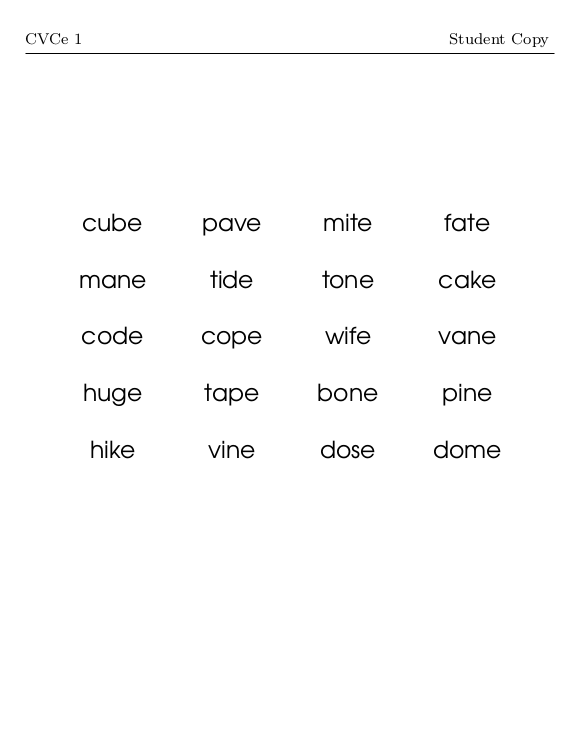
\includegraphics[width=6cm]{thumb1.png}};
\node[rotate=-10,line width=1mm,inner sep=0pt,draw=black] at (8,-14) {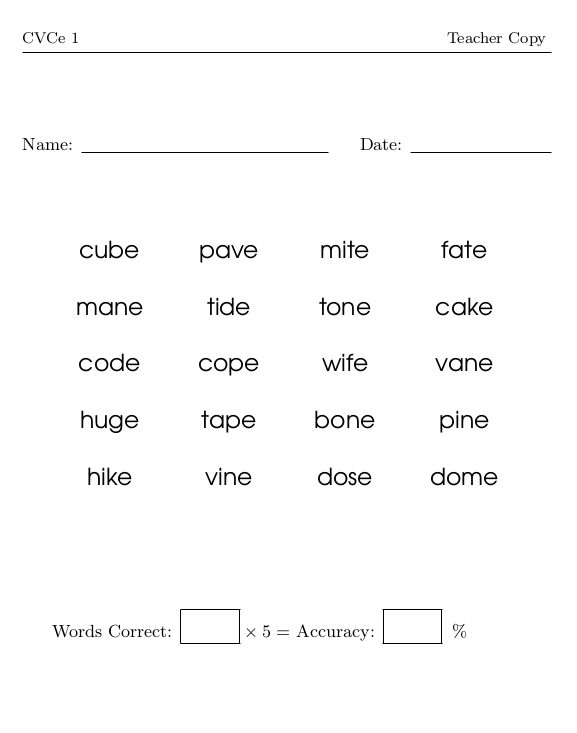
\includegraphics[width=6cm]{thumb2.png}};



\end{tikzpicture}


\end{document}
